% !TEX encoding = UTF-8 Unicode

\documentclass{article}
\usepackage[french]{babel}
\author{Louis DESVERNOIS, Alexis SCHOENN, Philippe DUBOIS}
\title{%
    SAÉ24: Réseau \\
    \large Groupe 13}
% \date{9 Juin 2022}
\usepackage[left=2.5cm,right=2.5cm,top=2.5cm,bottom=2.5cm]{geometry}
\usepackage{subcaption}
\usepackage{listings}
\usepackage{minted}
\usepackage{graphicx}
\usepackage[T1]{fontenc}
\usepackage[colorlinks=true,linkcolor=black,anchorcolor=black,citecolor=black,filecolor=black,menucolor=black,runcolor=black,urlcolor=black]{hyperref}
%\setcounter{tocdepth}{1} % pour la profondeur de la ToC

\usepackage{fancyhdr}
\pagestyle{fancy}
\fancyhf{}
\renewcommand{\headrulewidth}{0pt}
\rfoot{\thepage}
\lfoot{SAÉ24: Groupe 13}

\renewcommand{\listoflistingscaption}{Table des codes}
\renewcommand{\listingscaption}{Code}

\begin{document}

\maketitle
\tableofcontents
\listoffigures
\listoflistings

\newpage
\section{Création des VLAN et routage inter-VLAN}
\subsection{VLANs}
Pour commencer nous avons dû créer quatre VLAN sur notre switch ainsi que de mettre en place le routage inter-VLAN. 
Nous avons donc d'abord créé ces VLAN avec les commandes ci-dessous.
\begin{listing}[H]
    \begin{minted}[breaklines]{text}
Switch(config)#int range fastEthernet 0/1-4
Switch(config-if-range)#sw mode access 
Switch(config-if-range)#sw access vlan 10
% Access VLAN does not exist. Creating vlan 10
    \end{minted}
    \caption{Création d'un VLAN}
    \label{reseau:switch:vlans}
\end{listing}
Nous avons répété les commandes en code \ref{reseau:switch:vlans} quatre fois en utilisant quatre interfaces par VLAN ainsi que les numéros 10, 20, 30 et 40. 
Nous avons ensuite donné des noms à ces VLAN avec les commandes \verb|vlan <no>| puis \verb|name <nom>| en mode configuration.

\begin{listing}[H]
    \begin{minted}[breaklines]{text}
VLAN Name                             Status    Ports
---- -------------------------------- --------- -------------------------------
1    default                          active    Fa0/17, Fa0/18, Fa0/19, Fa0/20
                                                Fa0/21, Fa0/22, Fa0/23, Fa0/24
                                                Gig0/1, Gig0/2
10   voix                             active    Fa0/1, Fa0/2, Fa0/3, Fa0/4
20   users                            active    Fa0/5, Fa0/6, Fa0/7, Fa0/8
30   server                           active    Fa0/9, Fa0/10, Fa0/11, Fa0/12
40   admin                            active    Fa0/13, Fa0/14, Fa0/15, Fa0/16
1002 fddi-default                     active    
1003 token-ring-default               active    
1004 fddinet-default                  active    
1005 trnet-default                    active    
    \end{minted}
    \caption{Résultats de "sh vlan brief"}
    \label{reseau:switch:sh-vlan}
\end{listing}

\subsection{Routage inter-VLAN}
Une fois les VLAN correctement crées, nous avons besoin de configurer le routage inter-VLAN en utilisant l'encapsulation dot1Q.
Pour cela, sur notre switch, nous avons choisi le port \verb|Fa0/24| comme port trunk.
\begin{listing}[H]
    \begin{minted}[breaklines]{text}
Switch(config)#int fastEthernet 0/24
Switch(config-if)#sw mode trunk 
Switch(config-if)#sw trunk allowed vlan 10,20,30,40
    \end{minted}
    \caption{Configuration du port trunk}
    \label{reseau:switch:trunk}
\end{listing}
Le trunk étant activé, nous pouvons à présent créer les interfaces virtuelles sur le routeur. Nous avons besoin d'en créer quatre, une par VLAN. 
Au niveau de nos adresses IP, étant le groupe 13, nous pouvons utiliser les réseaux \verb|172.113.x.0/24| avec \verb|x| le numéro de VLAN. Les adresses choisies pour les gateways et les SVI seront respectivement la dernière et l'avant-dernière adresse de chaque réseau.
\begin{listing}[H]
    \begin{minted}[breaklines]{text}
interface FastEthernet0/0
    no ip address
!
interface FastEthernet0/0.10
    encapsulation dot1Q 10
    ip address 172.113.10.254 255.255.255.0
!
interface FastEthernet0/0.20
    encapsulation dot1Q 20
    ip address 172.113.20.254 255.255.255.0
!
interface FastEthernet0/0.30
    encapsulation dot1Q 30
    ip address 172.113.30.254 255.255.255.0
!
interface FastEthernet0/0.40
    encapsulation dot1Q 40
    ip address 172.113.40.254 255.255.255.0
    \end{minted}
    \caption{Création des interfaces virtuelles sur le routeur}
    \label{router:sub-int}
\end{listing}
Nous pouvons également en profiter pour configurer l'interface connectée à Internet en DHCP avec la commande \verb|ip address dhcp| en mode configuration d'interface.
\begin{figure}[H]
    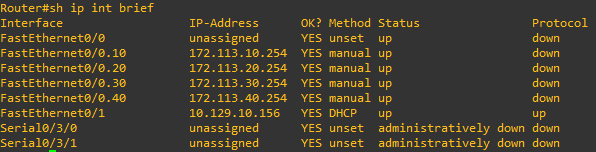
\includegraphics[width=\linewidth]{fig/router-dhcp.png}
    \caption{sh ip int brief}
    \label{router:shipintbrief}
\end{figure}
Comme nous pouvons le voir en Figure \ref{router:shipintbrief}, le routeur à bien récupéré une adresse IP avec DHCP et nous interfaces virtuelles ont correctement été configurées\footnote{Le protocole et en "down" sur Fa0/0 car au moment de la prise de la capture d'écran, un câble cassé étais utilisé}.  
\end{document}